\documentclass{article}
\usepackage[margin=1in]{geometry}
\usepackage{amsmath,amsfonts,amssymb}
\usepackage{listings}
\usepackage{color}
\usepackage{graphicx}
\usepackage{subfig}
\usepackage{blkarray}
\usepackage{multirow}
\usepackage{float}
\usepackage{caption}
\usepackage{subcaption}
\usepackage{dcolumn}
\usepackage{booktabs}
\usepackage{tikz}
\usetikzlibrary{positioning,shapes,arrows}
\newcolumntype{P}[1]{>{\centering\arraybackslash}p{#1}}
\newcolumntype{M}[1]{D{.}{.}{1.#1}}
\captionsetup[sub]{}

\definecolor{dkgreen}{rgb}{0,0.6,0}
\definecolor{gray}{rgb}{0.5,0.5,0.5}
\definecolor{mauve}{rgb}{0.58,0,0.82}

\newcommand\tab[1][1cm]{\hspace*{#1}}
\begin{document}
\begin{titlepage}
	\setlength{\parindent}{0pt}
	\large

\vspace*{-2cm}


\lstset{frame=tb,
  language=Python,
  aboveskip=3mm,
  belowskip=3mm,
  showstringspaces=false,
  columns=flexible,
  basicstyle={\small\ttfamily},
  numbers=none,
  numberstyle=\tiny\color{gray},
  keywordstyle=\color{blue},
  commentstyle=\color{dkgreen},
  stringstyle=\color{mauve},
  breaklines=true,
  breakatwhitespace=true,
  tabsize=3
}

University of Waterloo \par
CS 486 \par
\vspace{0.05cm}
r2knowle: 2023-11-11
\vspace{0.2cm}

{\huge Assignment \# 3 \par}
\hrule

\vspace{0.5cm}
\textbf{Q1.1)} To begin, we get the following diagram for the Naive Bayes Model based on the attributes of eating soup on days 1,2 and 3:\\
\begin{center}
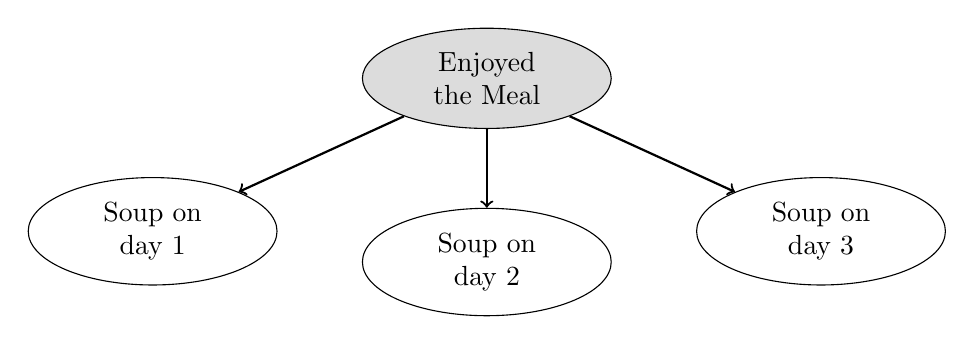
\begin{tikzpicture}[
  node distance=1cm and 2cm,
  mynode/.style={draw,ellipse,text width=2cm,align=center}]
\node[mynode,  fill={rgb,255:red,220; green,220; blue,220}] (en) {Enjoyed the Meal};
\node[mynode, below left=of en] (s1) {Soup on day 1};
\node[mynode, below=of en] (s2) {Soup on day 2};
\node[mynode, below right=of en] (s3) {Soup on day 3};


\path[->,draw,thick]
  (en) edge  (s1)
  (en) edge  (s2)
  (en) edge  (s3);
 
\end{tikzpicture}
\end{center}
From this we can get the derive the following thetas:
\begin{align*}
\theta &= \text{P(C=True)} \\
\theta_{1,1} &= \text{P(Soup on day 1 = True } |\text{ C = True)} \\
\theta_{1,2} &= \text{P(Soup on day 1 = True } |\text{ C = False)} \\
\theta_{2,1} &= \text{P(Soup on day 2 = True } |\text{ C = True)} \\
\theta_{2,2} &= \text{P(Soup on day 2 = True } |\text{ C = False)} \\
\theta_{3,1} &= \text{P(Soup on day 3 = True } |\text{ C = True)} \\
\theta_{3,2} &= \text{P(Soup on day 3 = True } |\text{ C = False)} \\
\end{align*}
After applying Lapace smoothing we get the following values for theta:
\begin{align*}
\theta = \frac{2+1}{5+2} = \frac{3}{7} 
\end{align*}
\begin{center}
\begin{tabular}{ll}
$\theta_{1,1} = \frac{2 + 1}{2 + 2} = \frac{3}{4}$  & $\theta_{1,2} = \frac{1+1}{3 + 2} = \frac{2}{5}$ \\\\
$\theta_{2,1} = \frac{2 + 1}{2 + 2} = \frac{3}{4}$  & $\theta_{2,2} = \frac{0+1}{3 + 2} = \frac{1}{5}$ \\\\\
$\theta_{3,1} = \frac{1 + 1}{2 + 2} = \frac{2}{4}$  & $\theta_{3,2} = \frac{2+1}{3 + 2} = \frac{3}{5}$ \\\\\
\end{tabular}
\end{center}
\textbf{Q1.2)} To solve we have 2 sets of 2 probabilities. In the case of having soup on day 1 we have (note Dx represents soup on day x):
\begin{align*}
P(\text{Enjoy Meal}  |D_1, \neg D_2, \neg D)3) &= \alpha \times \theta \times \theta_{1,1} \times (1-\theta_{2,1}) \times (1-\theta_{3,1}) \\
&= \frac{3}{7} \times \frac{3}{4} \times \frac{1}{4} \times \frac{1}{2} \\
&= \frac{9}{224}
\end{align*}
\begin{align*}
P(\text{Didnt Enjoy Meal}  |D_1, \neg D_2, \neg D)3) &= \alpha \times (1-\theta) \times \theta_{1,2} \times (1-\theta_{2,2}) \times (1-\theta_{3,2}) \\
&= \frac{4}{7} \times \frac{2}{5} \times \frac{4}{5} \times \frac{2}{5} \\
&= \frac{64}{875}
\end{align*}
In comparison, if we have soup on both days 1 and 2 we get the following probabilities:
\begin{align*}
P(\text{Enjoy Meal}  |D_1, D_2, \neg D)3) &= \alpha \times \theta \times \theta_{1,1} \times \theta_{2,1} \times (1-\theta_{3,1}) \\
&= \frac{3}{7} \times \frac{3}{4} \times \frac{3}{4} \times \frac{1}{2} \\
&= \frac{27}{224}
\end{align*}
\begin{align*}
P(\text{Didnt Enjoy Meal}  |D_1, D_2, \neg D)3) &= \alpha \times (1-\theta) \times \theta_{1,2} \times \theta_{2,2} \times (1-\theta_{3,2}) \\
&= \frac{4}{7} \times \frac{2}{5} \times \frac{1}{5} \times \frac{2}{5} \\
&= \frac{16}{875}
\end{align*}
Therefore we can see that the probability Alex enjoys his meal goes up if he had soups on day 1 and 2, as well as his probability for not liking the meal also goes down. Therefore we can conclude he is more likely to like his meal is he has soups on both days 1 and 2.
\newpage
\textbf{Q2.1)} As taught in class we know the expected value is equal to:
\[ \text{Expected Value} = \sum_s P(s)U(s) \]
In our case we get that this is equivalent to:
\begin{align*}
\text{Expected Value} &= \sum^\infty_{i=1} \frac{1}{2^i}\times2^i \\
&= \sum^\infty_{i=1} 1 \\
&= \infty
\end{align*}
Thus showing the expected value of this game is infinite.\\\\
\textbf{Q2.2)} If I could play the game regardless of how much I bid, I would always only pay $0$ as that would maximize my utility of winning, otherwise I would pay a maximum of $100$ :).\\\\
\textbf{Q2.3)} Given this new utility function we get that the expected utility is:
\begin{align*}
\text{Expected Uility} &= \sum^\infty_{i=1} \frac{1}{2^i}\times(a\log_2(2^i) + b) \\
&= a\sum^\infty_{i=1}(\frac{i}{2^i}) + b\sum^\infty_{i=1}(\frac{1}{2^i})\\
&= a\sum^\infty_{i=1}(\frac{i}{2^i}) + b\sum^\infty_{i=1}(\frac{1}{2})^i
\end{align*}
Note that the right equation is equivalent to the geometric series with $x = \frac{1}{2}$ (starting at the second term) and so we get:
\begin{align*}
&= a\sum^\infty_{i=1}(\frac{i}{2^i}) + b (\frac{1}{1-\frac{1}{2}}-1) \\
&= a \left(\frac{1}{2} + \frac{2}{4} + \frac{3}{8} + \frac{4}{16} + ... \right) + b \\
&= 2a + b
\end{align*}
Thus we get that the expected utility from playing this game is equal to 2a + b.\\\\
\textbf{Q2.4)} To begin we can get that our expected utility is:
\[ \text{Expected Utility} = 2a + b \]
Moreover the utility of money we get is equal to the money we earn - the price we needed to bid. Lets assume that our bid is equal to our entire wealth. Thus we get:
\begin{align*}
 a\log_2(k-x)+b &= 2a + b\\
 \log_2(k-x) &= 2\\
 k-x &= 4\\
 -x &= 4-k\\
 x &= k-4\\
\end{align*}
Therefore we have that x = k-4.
\newpage
\textbf{Q3.1a)} Before we determine the optimal policy give a specific risk probability, we will first determine the value function for each action. Starting with action a we have the following value functions for each state:

\newpage
\textbf{Q4.1)} Below is the code used to produce the decision tree, as well as get the number of values predicted correctly vs incorrectly:
\begin{lstlisting}
import numpy as np

# ============= Loss Implementation =============
def entropyLoss(vals_y):

    count = 0.0
    for val in vals_y:
        if val == "healthy.\n":
            count += 1.0
    p = 0
    if count != 0:
        p = count / float(len(vals_y))

    if p == 1 or p == 0:
        return 0

    return -p * np.log2(p) - (1 - p) * np.log2(1 - p)

# ============= Decision Tree Implementation =============

class DecisionTree:
    threshold = 0
    thresholdFeature = 0
    values = []
    leftTree = -1
    rightTree = -1
    classification = 0
    numLeft = 0
    numRight = 0
    counter = 0

    # This method determines if all values are homogenous
    def allTheSame(self, vals):
        if len(vals) == 0:
            return True
        originalValue = vals[0][-1]
        for val in vals:
            if (val[-1] != originalValue):
                return False
        return True


    # Given a dataset, this function will determine where the split is to minimize entropy loss (maximize info gain)
    def findBestThreshold(self, vals, loss):
        bestLoss = 9999999
        bestFeature = 0
        bestThreshold = 0

        width = len(vals[0]) - 1
        for test_entry in vals:
            for idx in range(0, width):
                left = []
                right = []

                for entry in vals:
                    # Note that picking a threshold that is <= two consecutive elements is the same as >= the top element.
                    #   as no elements by definition can be between the threshold and the proposed threshold
                    if (float(entry[idx]) >= float(test_entry[idx])):
                        right.append(entry[-1])
                    else:
                        left.append(entry[-1])

                leftWeight = len(left) / (len(left) + len(right))
                rightWeight = len(right) / (len(left) + len(right))

                totalLoss = loss(left) * leftWeight + loss(right) * rightWeight
                if totalLoss < bestLoss:
                    bestLoss = totalLoss
                    bestFeature = idx
                    bestThreshold = test_entry[idx]

        return [bestFeature, bestThreshold]

    def __init__(self, vals, loss):
        if self.allTheSame(vals):
            self.values = vals
        else:
            x = self.findBestThreshold(vals, loss)
            self.thresholdFeature = x[0]
            self.threshold = x[1]

            leftTreeVals = []
            rightTreeVals = []
            for val in vals:
                if float(val[self.thresholdFeature]) >= float(self.threshold):
                    rightTreeVals.append(val)
                else:
                    leftTreeVals.append(val)

            self.leftTree = DecisionTree(leftTreeVals, loss)
            self.rightTree = DecisionTree(rightTreeVals, loss)

    def classify(self, item):
        if self.leftTree == -1:
            if item[-1] == self.values[0][-1]:
                return 1
            print(item[-1])
            return 0
        else:
            if float(item[self.thresholdFeature]) >= float(self.threshold):
                return self.rightTree.classify(item)
            return self.leftTree.classify(item)

    def printTree(self, indx, cols):
        if len(self.values) == 0:
            print("LV ", indx, ": ", cols[self.thresholdFeature], " ", self.threshold)
        else:
            print("LV", indx, ": ", self.values[0][-1].split("\n")[0])
        if self.leftTree != -1:
            self.leftTree.printTree(indx+1, cols)
        if self.rightTree != -1:
            self.rightTree.printTree(indx+1, cols)

    def predict(self, items):
        count = 0
        for val in items:
            count += self.classify(val)
        return count


# ============= Testing of Values =============

trainingFile = open("horseTrain.txt", "r")
lines = trainingFile.readlines()
training = []
for line in lines:
    training.append(line.split(","))

columns = ["K", "Na", "CL", "HCO3", "Endotoxin", "Aniongap", "PLA2", "SDH", "GLDH", "TPP", "Breath rate",
           "PCV", "Pulse rate", "Fibrinogen", "Dimer", "FibPerDim"]

dt = DecisionTree(training, entropyLoss)
dt.printTree(1, columns)
print("Correct Predictions:", dt.predict(training),  "out of", len(training))

testFile = open("horseTest.txt", "r")
lines = testFile.readlines()
testing = []
for line in lines:
    testing.append(line.split(","))
print("Correct Predictions:", dt.predict(testing),  "out of", len(testing))
\end{lstlisting}
\textbf{Q4.2)} This gives us the following decision tree:\\\\

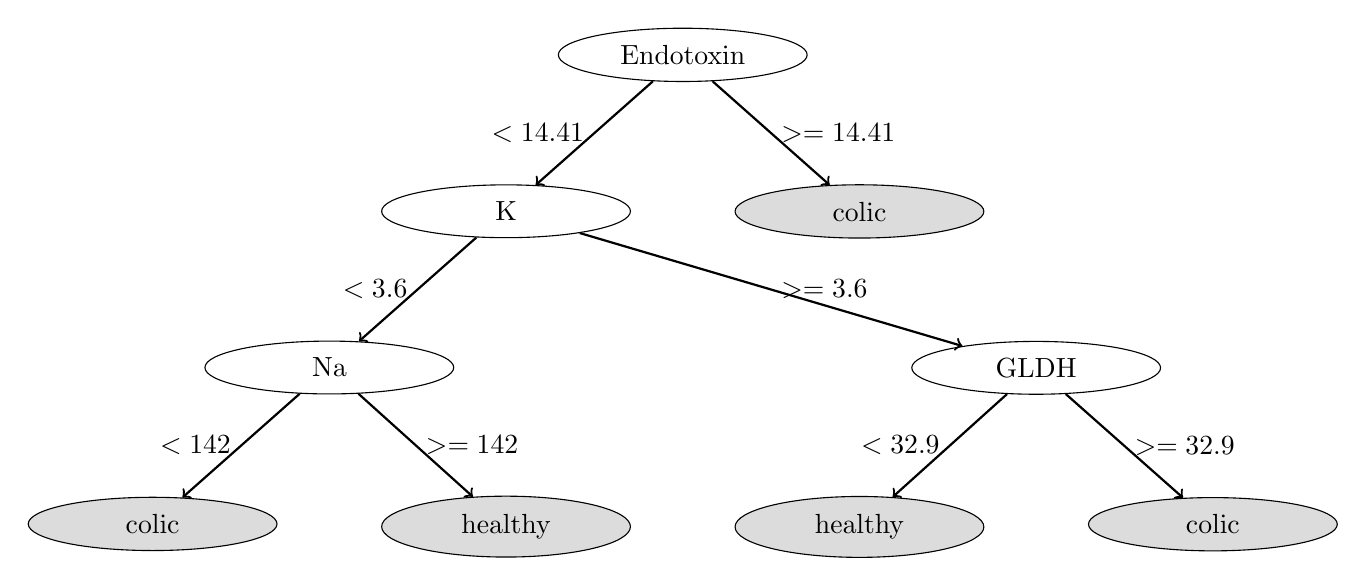
\begin{tikzpicture}[
  node distance=1.5cm and 0cm,
  mynode/.style={draw,ellipse,text width=2cm,align=center}]
\node[mynode] (en) {Endotoxin};
\node[mynode, below left=of en] (k) {K};
\node[mynode,  fill={rgb,255:red,220; green,220; blue,220}, below right=of en] (2c) {colic};
\node[mynode, below left=of k] (na) {Na};
\node[mynode, below right=of 2c] (gldh) {GLDH};
\node[mynode, fill={rgb,255:red,220; green,220; blue,220}, below left=of na] (4c) {colic};
\node[mynode, fill={rgb,255:red,220; green,220; blue,220}, below right=of na] (4h) {healthy};
\node[mynode, fill={rgb,255:red,220; green,220; blue,220}, below left=of gldh] (4hr) {healthy};
\node[mynode, fill={rgb,255:red,220; green,220; blue,220}, below right=of gldh] (4cr) {colic};


\path[->,draw,thick]
  (en) edge node[left=of en] {$< 14.41$} (k)
  (en) edge node[right=of en] {$>= 14.41$} (2c)
  (k) edge node[left=of en] {$< 3.6$} (na)
  (k) edge node[right=of en] {$>= 3.6$} (gldh)
  (na) edge node[left=of en] {$< 142$} (4c)
  (na) edge node[right=of en] {$>= 142$} (4h)
  (gldh) edge node[left=of en] {$< 32.9$} (4hr)
  (gldh) edge node[right=of en] {$>= 32.9$} (4cr);
 
\end{tikzpicture}
\newpage
\textbf{Q4.3)} For the training set we get that we correctly classifiy:
\[ \text{132 out of 132 training data points} \]
\textbf{Q4.4)} For the test set we get that we correctly classify:
\[ \text{13 our of the 13 testing data points} \]
\end{titlepage}
\end{document}